%%%%%%%%%%%%%%%%%%%%%%%%%%%%%%%%%%%%%%%%%
% Short Sectioned Assignment
% LaTeX Template
% Version 1.0 (5/5/12)
%
% This template has been downloaded from:
% http://www.LaTeXTemplates.com
%
% Original author:
% Frits Wenneker (http://www.howtotex.com)
%
% License:
% CC BY-NC-SA 3.0 (http://creativecommons.org/licenses/by-nc-sa/3.0/)
%
%%%%%%%%%%%%%%%%%%%%%%%%%%%%%%%%%%%%%%%%%

%----------------------------------------------------------------------------------------
%	PACKAGES AND OTHER DOCUMENT CONFIGURATIONS
%----------------------------------------------------------------------------------------

\documentclass[paper=a4, fontsize=11pt]{scrartcl} % A4 paper and 11pt font size

\usepackage[T1]{fontenc} % Use 8-bit encoding that has 256 glyphs
\usepackage{fourier} % Use the Adobe Utopia font for the document - comment this line to return to the LaTeX default
\usepackage[english]{babel} % English language/hyphenation
\usepackage{amsmath,amsfonts,amsthm} % Math packages
\usepackage[pdftex]{graphicx}
\graphicspath{{./}}

\usepackage{lipsum} % Used for inserting dummy 'Lorem ipsum' text into the template
\usepackage{float} % set the figures precisely

\usepackage{sectsty} % Allows customizing section commands
\allsectionsfont{\centering \normalfont\scshape} % Make all sections centered, the default font and small caps

\usepackage{fancyhdr} % Custom headers and footers
\pagestyle{fancyplain} % Makes all pages in the document conform to the custom headers and footers
\fancyhead{} % No page header - if you want one, create it in the same way as the footers below
\fancyfoot[L]{} % Empty left footer
\fancyfoot[C]{} % Empty center footer
\fancyfoot[R]{\thepage} % Page numbering for right footer
\renewcommand{\headrulewidth}{0pt} % Remove header underlines
\renewcommand{\footrulewidth}{0pt} % Remove footer underlines
\setlength{\headheight}{13.6pt} % Customize the height of the header

\numberwithin{equation}{section} % Number equations within sections (i.e. 1.1, 1.2, 2.1, 2.2 instead of 1, 2, 3, 4)
\numberwithin{figure}{section} % Number figures within sections (i.e. 1.1, 1.2, 2.1, 2.2 instead of 1, 2, 3, 4)
\numberwithin{table}{section} % Number tables within sections (i.e. 1.1, 1.2, 2.1, 2.2 instead of 1, 2, 3, 4)

\usepackage{tikz} % Draw graph library

%\setlength\parindent{0pt} % Removes all indentation from paragraphs - comment this line for an assignment with lots of text

%----------------------------------------------------------------------------------------
%	TITLE SECTION
%----------------------------------------------------------------------------------------

\newcommand{\horrule}[1]{\rule{\linewidth}{#1}} % Create horizontal rule command with 1 argument of height

\title{	
\normalfont \normalsize 
\textsc{Network Virtualization and Data Center Networks} \\ [25pt] % Your university, school and/or department name(s)
\horrule{0.5pt} \\[0.4cm] % Thin top horizontal rule
\huge Assignment 2: Cloud computing - software engineer perspective\\ % The assignment title
\horrule{2pt} \\[0.5cm] % Thick bottom horizontal rule
}

\author{Erik Henriksson, Christoph Burkhalter} % Your name

\date{\normalsize\today} % Today's date or a custom date

\begin{document}

\maketitle % Print the title

\section{Part A - Proposal}

\subsection{Application}


We will use a simple web-server scenario for the benchmarking and the auto-scaling. There are two types of machines: load-balancers and worker machines. The load-balancers get an IP from a predefined pool of Elastic-IP's such that requests from clients can be sent to them. All load-balancers connect to the overlay network and receive the list of worker machines from the coordinator. Incoming request are sent to a worker machine using a load-balancing technique. In this way load-balancers are connected to all machines in the network, whereas worker machines are only connected to the load-balancers.
The worker machines process the request and contain no further application logic, which means they are not members of the overlay network.
The members of the overlay network (the load-balancers) elect a coordinator and perform a re-electing in case the coordinator dies. We will study the case with exactly two load-balancers, but it is of course easy to scale this up.

\tikzset{
  treenode/.style = {align=center, inner sep=0pt, text centered,
    font=\sffamily},
  load_balancer/.style = {circle, text=white, draw=none,fill=blue},
  node/.style = {circle, text=black, draw=black},
}

\begin{figure}[H]
\begin{center}
\begin{tikzpicture}[node distance=1cm]
  
  \node [load_balancer] (l1) at (1,2) {L1};
  \node [load_balancer] (l2) at (3,2) {L2};
  \node [node] (n1) at (0,0)  {W1};
  \node [node] (n2) at (2,0) {W2};
  \node [node] (n3) at (4,0)  {W3};

  \foreach \from/\to in {l1/l2,l1/n1,l1/n2,l1/n3,l2/n1,l2/n2,l2/n3}
    \draw (\from) -- (\to);

\end{tikzpicture}
\end{center}

\caption{Network with load balancers (L1,L2) and processing nodes (W1,W2,W3)}
\end{figure}

\subsection{Benchmark}

The benchmark contains latency measurements between machines in the Amazon cloud (cloud to cloud), and a latency test of the application from a client outside the Amazon cloud (client to cloud). The benchmark will be initiated by the coordinator and executed on each machine for the performance benchmark. The latency benchmark is performed on the load-balancers; they test the latency on the network to all running machines in the cloud (other load balancers as well as all the worker machines). These results will be used to optimize load-balancing as well as for the auto scaling.
Additionally,the performance of the system is benchmarked by various workloads (e.g. 1000 request per second from a client). These benchmarks test will be performed with different numbers of worker machines, but a fixed number of two load-balancers.

\subsection{Auto-scaling}

The coordinator in the load balancer network performs the auto-scaling. If the load on the worker machines is too large, the coordinator will start new machines (scale-out). For the scale-out there will be a snapshot with the installed application to improve the start-up time. 
If the workload decreases, the reverse will be done.
In this part we will compare the Amazon load-balancer with our own implementation of a load-balancer, where we detect heavy-loaded machines if the latency increases or from periodically sending ping messages.

\section{Part B and C - Implementation}

We have used the twisted library in python and found a open source load balancer named \verb|txLoadBalancer| to do our implementation. It had functions for proxying requests, scheduling the processing nodes and working as a reverse proxy. To this we added the overlay code, code for measuring the request processing time and code to scale up and down the processing nodes.

\subsection{Overlay}
Our overlay network consists of a coordinator load balancer and slave load balancers. The coordinator is responsible for the autoscaling of the network and maintaining of the overlay, otherwise the load balancers are identical. Note that the processing nodes is not part of the overlay, they are not aware of anything else than process incoming requests from the load balancers. The overlay nodes has currently not any ability to start or stop each other, it is purely a this of redundancy. With this said, a couple of these load balancers can tolerate a very high number of requests per second and bottleneck should not be the load balancers. A couple of load balancers are also "cheap", whereas a huge number of processing nodes are not. We can therefore use use a safe margin when we dimension the number of load balancers without this having any important impact on the budget.

\subsection{Request processing time}
To get a good measurement of the network load we need to use a way to measure the amount of incoming request combined with their difficulty to process. A problem that arises here is that we can not assume anything of the distribution of request to different load balancers, and measuring at all of them is hard to synchronize. Therefore, we chose to measure the average processing time, since this is dependant on both the difficulty to process and the amount of requests. It is also very easy to measure at a central location, i.e. the coordinator load balancer. 

To avoid the problem when the load balancer does not get any reguests (and therefore can't calculate an average) we send dummy requests from the coordinator load balancer. The average is then calculated as
$$\frac{1}{N}\sum^N_{i=1} T_i$$
where $T_i$ is an exponential moving average of the request processing time at processing node $i$ and $N$ is the number of processing nodes.
\subsection{Autoscaling}
We use, as noted before, the average request processing time to determine when to scale up or down the processing node. It is the coordinator load balancer that is responsible for this, and it will have to config parameters to determine this, namely the scale-down parameter \verb|scale_down| and the scale-up parameter \verb|scale_up|. It simply compares the current average with the parameters and scales up if current average is above the \verb|scale_up| parameter. Scale down is done in the opposite way. On each scale we do doubling or halving of the network to achieve a certain size in $log(n)$ steps. It can therefore scale up or down very fast and will tolerate very fast changes in load without failing requests.

\section{Problems}
We noticed a couple of problems during our experiments on the Amazon EC2 cloud. We noticed that a start-up of a node can take up to 60 seconds, something that has impact on the speed of scaling. This problem can be seen in the graphs, where the load balancer sees a high load and initiates a scale up but it takes up to 60 seconds for this to take effect. 

We also had problems with CPU throttling on the micro instances, where you are granted a "free" CPU burst for some minutes and then restricted to a very low amount of CPU. This makes the average request processing time skyrocket even faster and the load balancer sees this as a increased load and scales up the nodes even faster. We therefore do not recommend running this on micro instances, it is better to use small instances where the CPU capacity is guaranteed over time.

\section{Results}

The average response time per request increases linear with the number of concurrent requests. This is due to the fact that the twisted framework runs the requests in parallel. For up to 200 concurrent requests, there is no indication of an overhead while handling that many requests. The figures for a micro and a small instance on the Amazon EC2 Cloud are very similar, the only difference is the response time, which is higher for the small instance. This is due to the fact that the micro instance has a burst mode, for a small amount of time the processing speed is much higher than the small instance. However, once this time is up, the processing speed drops significantly below the value of the small instance. 

\begin{figure*}[h!]
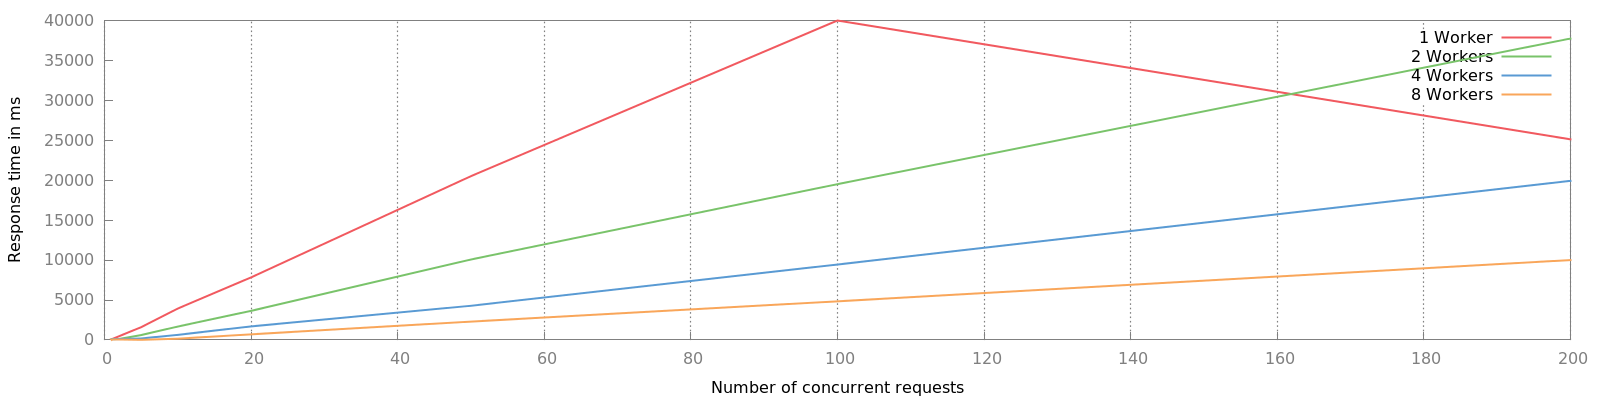
\includegraphics[width=\columnwidth]{../plot/latency_fixed.png}
\end{figure*}

\begin{figure*}[h!]
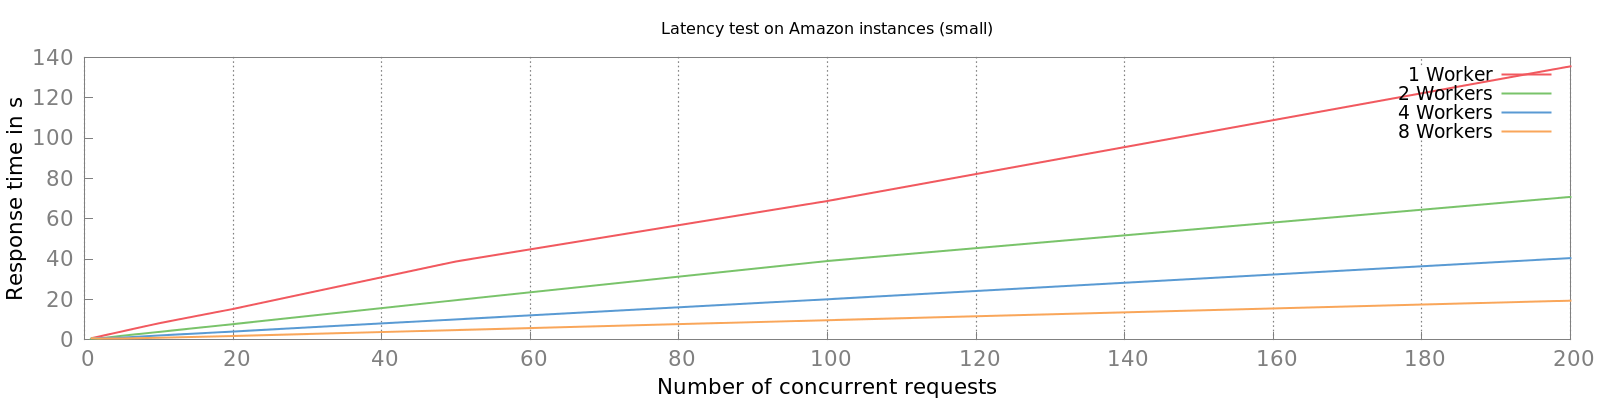
\includegraphics[width=\columnwidth]{../plot/latency_fixed_small.png}
\end{figure*}

The number of processed request is calculated from the average response time per request. As expected, for one concurrent request the response time and therefore the throughput are almost identical. However, with twice as many worker server machines, the number of processed requests per second almost doubles as well. For example on a small instance, 2 worker server process on average about 2.5 requests per second, where 4 worker server are able to process about 5 requests per second.

\begin{figure*}[h!]
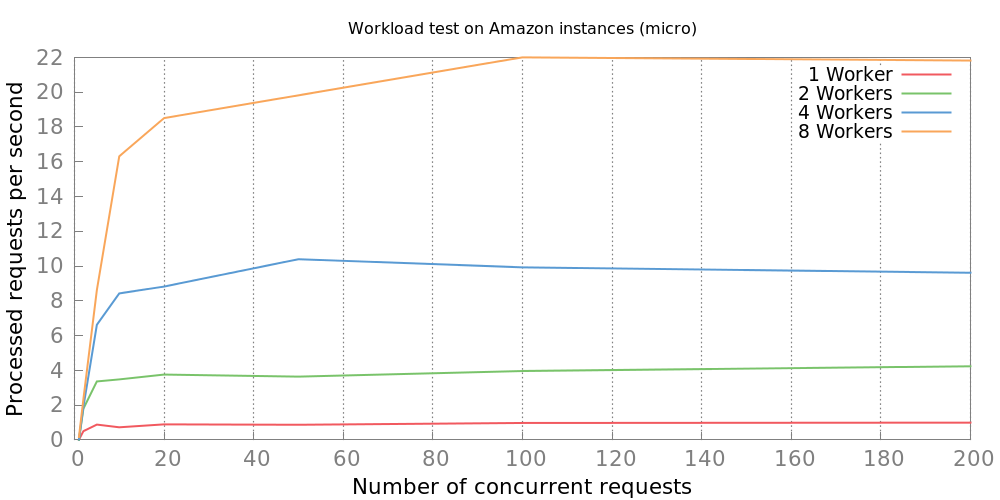
\includegraphics[width=\columnwidth]{../plot/workload.png}
\end{figure*}

\begin{figure*}[h!]
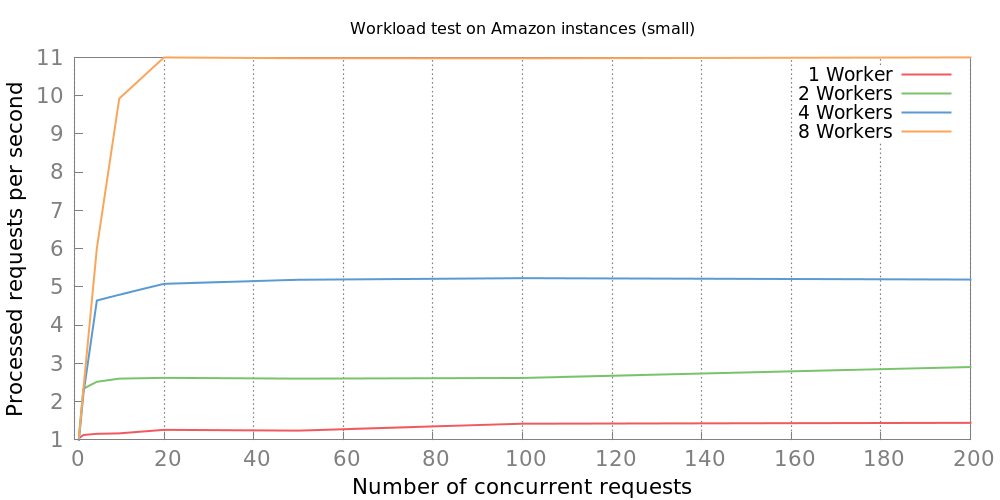
\includegraphics[width=\columnwidth]{../plot/workload_small.png}
\end{figure*}

The latency test measures the response time per request over a period of 5 minutes with 50 concurrent requests. Whenever a requests finished, a new one was started such that the system had always the same amount of workload.
Unfortunately, we run out of time and therefore weren't able to perform the test with 1 Worker on an Amazon micro instance.

The lines for a fixed number of workers have a small fluctuation around a average response time. With a longer running time, the fluctuation increases on the micro instance. For the auto-scaling part the response time start at a high level and drops around 150 seconds on both micro and small instances. On the small instance it has then the shortest response time and is very stable, while on the micro instance there is a high fluctuation. Even though the auto-scaling starts more than 8 new servers, there is only one signification drop in the line. So after a long initialization phase the machines start there work closely after each other. For the auto-scaling on small instances, the significant drop descends to a response time of around 10 seconds, and then it decreases in small steps until it is below 5 seconds. So there seem to be more machines starting their work. This is due to the fact that the first machine doubles the processing power, while when the system has for example 8 worker servers and a new one joins the system, the processing power gets only a small improvement.

\begin{figure*}[h!]
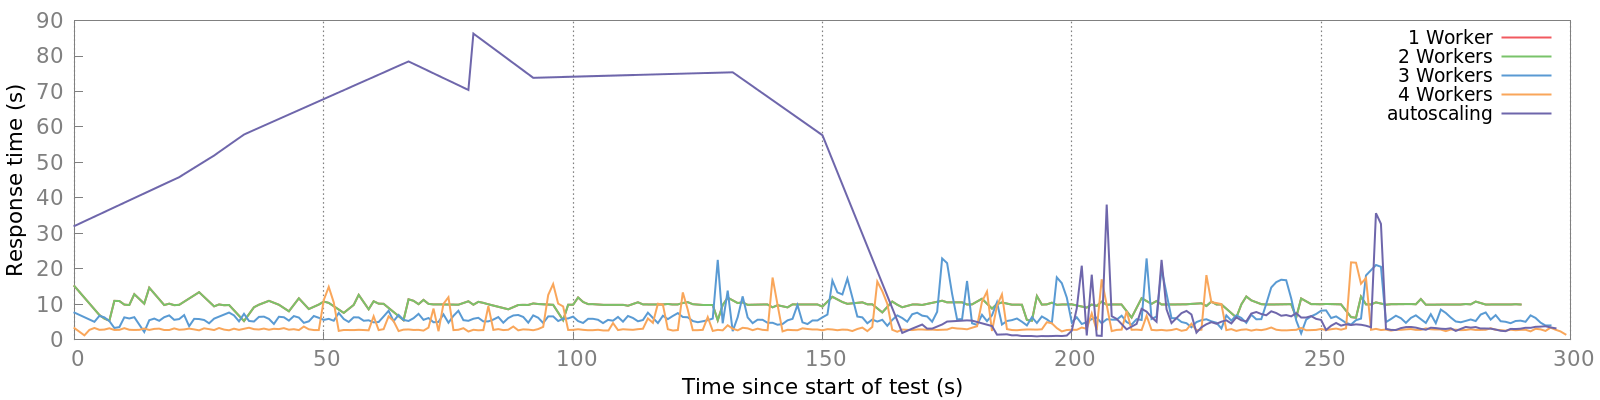
\includegraphics[width=\columnwidth]{../plot/timeline.png}
\end{figure*}

\begin{figure*}[h!]
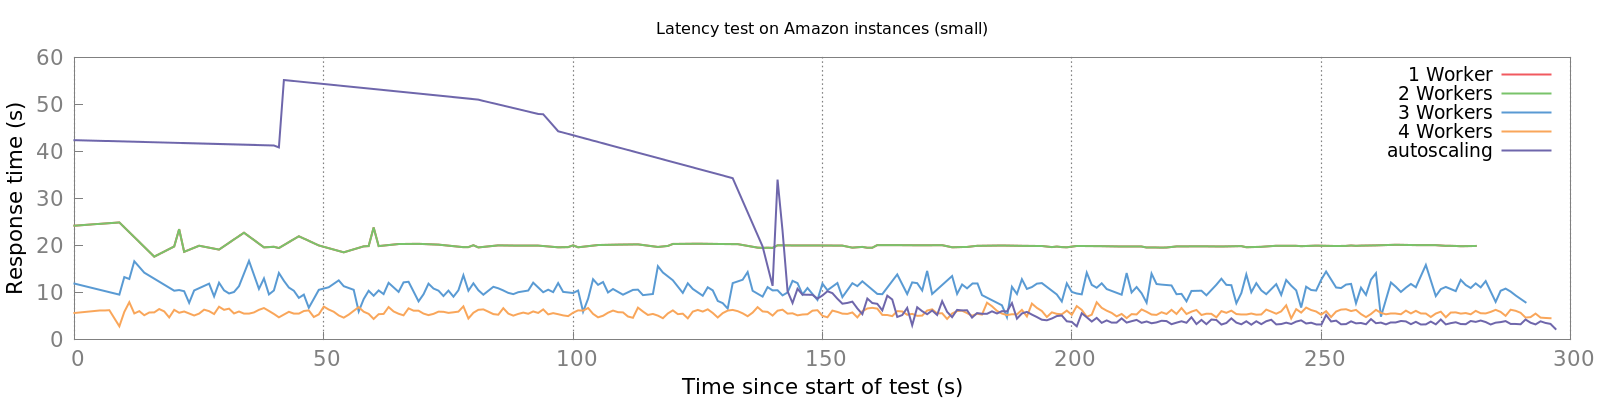
\includegraphics[width=\columnwidth]{../plot/timeline_small.png}
\end{figure*}

\newpage

\section{Part D - Billing}

\subsection{Scenario}

Estimate the cost for hosting a small business using the public-cloud of Amazon or Microsoft or having it in-house. The goal is to find the cheapest configuration that fullfills all requirements, which are:

\begin{itemize}
	\item 1 web server - hosting everything (Suse Linux Enterprise 64 bit, 4 CPUs, 8GB RAM)
	\item 1 TB storage
	\item 10 GB / week data transfer
	\item SLES - SUSE Linux Enterprise Server - system type
\end{itemize}

\subsection{Comparison}

The comparison is made for the US market, therefore all prices are US dollars.
Amazon provides a Free Tier Discount for the first year (1.68\$ per month) and discount for long term reservations with payment upfront.

\begin{itemize}
	\item Amazon: 4 CPU, 15 GB RAM, 1680 GB Storage, 10 GB / week (m1.xlarge)
	\item Windows Azure : 8x1.6GHz CPU, 14 GB RAM, 2040 GB Storage, 44 GB / month (XL Linux)
	\item IBM (in-house and SmartCloud): 4 CPU, 8 GB RAM, 1084 GB Storage, 10 GB / week (64-bit Silver)
\end{itemize}

\begin{table}
	\centering
	\begin{tabular}{| l | r | r | r |}
		\hline
		& 1 Month & 1 Year & 3 Years \\
		\hline
		Amazon & 427.92 & 2657.18 & 5309.96 \\
		\hline
		Azure & 361.80 & 4341.60 & 13071.60 \\
		\hline
		In-house & 5570.00 & 12093.00 & 26325.00 \\
		\hline
		SmartCloud & 250.00 & 3000.00 & 9000.00 \\
		\hline
	\end{tabular}
	\caption{Price comparison public-cloud, in-house. All values in \$.}
	\label{tab:pricetable}
\end{table}


The IBM SmartCloud is the cheapest for a short time of usage. However, it has the advantage to match the requirements accurately. Amazon gets huge discounts for a long reservation, it is the cheapest in the long run. Additionally, the virtual machine provides almost twice as much RAM as requested and more than 1.5 times the amount of storage. Windows Azure is the most expensive cloud solution, but this is partly due to the fact that it offers almost twice as many CPU,RAM and storage. A cheaper virtual machine that fits the requirements except the RAM (only 7 GB) costs below 190\$ per month and would be the cheapest. Of course, this could be done for Amazon as well, reducing the price for a month below 250\$. So while it is arguably which vendor is the cheapest in a short run, Amazon is definitely the best choice for a longer period. The in-house estimate has an capital investment of 4977\$ and a high 593\$ monthly cost. So even after the first investment, the in-house solution has the highest maintenance costs.



\end{document}
